% THIS IS SIGPROC-SP.TEX - VERSION 3.1
% WORKS WITH V3.2SP OF ACM_PROC_ARTICLE-SP.CLS
% APRIL 2009
%
% It is an example file showing how to use the 'acm_proc_article-sp.cls' V3.2SP
% LaTeX2e document class file for Conference Proceedings submissions.
% ----------------------------------------------------------------------------------------------------------------
% This .tex file (and associated .cls V3.2SP) *DOES NOT* produce:
%       1) The Permission Statement
%       2) The Conference (location) Info information
%       3) The Copyright Line with ACM data
%       4) Page numbering
% ---------------------------------------------------------------------------------------------------------------
% It is an example which *does* use the .bib file (from which the .bbl file
% is produced).
% REMEMBER HOWEVER: After having produced the .bbl file,
% and prior to final submission,
% you need to 'insert'  your .bbl file into your source .tex file so as to provide
% ONE 'self-contained' source file.
%
% Questions regarding SIGS should be sent to
% Adrienne Griscti ---> griscti@acm.org
%
% Questions/suggestions regarding the guidelines, .tex and .cls files, etc. to
% Gerald Murray ---> murray@hq.acm.org
%
% For tracking purposes - this is V3.1SP - APRIL 2009

\documentclass{acm_proc_article-sp}

\begin{document}

\title{TITLE
Format\titlenote{(Does NOT produce the permission block, copyright information nor page numbering). For use with ACM\_PROC\_ARTICLE-SP.CLS. Supported by ACM.}}
\subtitle{[Extended Abstract]
\titlenote{A full version of this paper is available as
\textit{Author's Guide to Preparing ACM SIG Proceedings Using
\LaTeX$2_\epsilon$\ and BibTeX} at
\texttt{www.acm.org/eaddress.htm}}}
%
% You need the command \numberofauthors to handle the 'placement
% and alignment' of the authors beneath the title.
%
% For aesthetic reasons, we recommend 'three authors at a time'
% i.e. three 'name/affiliation blocks' be placed beneath the title.
%
% NOTE: You are NOT restricted in how many 'rows' of
% "name/affiliations" may appear. We just ask that you restrict
% the number of 'columns' to three.
%
% Because of the available 'opening page real-estate'
% we ask you to refrain from putting more than six authors
% (two rows with three columns) beneath the article title.
% More than six makes the first-page appear very cluttered indeed.
%
% Use the \alignauthor commands to handle the names
% and affiliations for an 'aesthetic maximum' of six authors.
% Add names, affiliations, addresses for
% the seventh etc. author(s) as the argument for the
% \additionalauthors command.
% These 'additional authors' will be output/set for you
% without further effort on your part as the last section in
% the body of your article BEFORE References or any Appendices.

\numberofauthors{8} %  in this sample file, there are a *total*
% of EIGHT authors. SIX appear on the 'first-page' (for formatting
% reasons) and the remaining two appear in the \additionalauthors section.
%
\author{
% You can go ahead and credit any number of authors here,
% e.g. one 'row of three' or two rows (consisting of one row of three
% and a second row of one, two or three).
%
% The command \alignauthor (no curly braces needed) should
% precede each author name, affiliation/snail-mail address and
% e-mail address. Additionally, tag each line of
% affiliation/address with \affaddr, and tag the
% e-mail address with \email.
%
% 1st. author
\alignauthor
Author1\titlenote{titlenote}\\
       \affaddr{Affiliation}\\
       \affaddr{affliation addr}\\
       \affaddr{affliation address}\\
       \email{email}
% 2nd. author
\alignauthor
Author2\titlenote{titlenote}\\
       \affaddr{Affiliation}\\
       \affaddr{affliation addr}\\
       \affaddr{affliation address}\\
       \email{email}
% 3rd. author
\alignauthor Author3\titlenote{titlenote}\\
       \affaddr{Affiliation}\\
       \affaddr{affliation addr}\\
       \affaddr{affliation address}\\
       \email{email}
\and  % use '\and' if you need 'another row' of author names
% 4th. author
\alignauthor  Author4\titlenote{titlenote}\\
       \affaddr{Affiliation}\\
       \affaddr{affliation addr}\\
       \affaddr{affliation address}\\
       \email{email}
% 5th. author
\alignauthor Author5\titlenote{titlenote}\\
       \affaddr{Affiliation}\\
       \affaddr{affliation addr}\\
       \affaddr{affliation address}\\
       \email{email}
% 6th. author
\alignauthor Author6\titlenote{titlenote}\\
       \affaddr{Affiliation}\\
       \affaddr{affliation addr}\\
       \affaddr{affliation address}\\
       \email{email}
}

\maketitle
\begin{abstract}
ABSTRACT
\end{abstract}

% A category with the (minimum) three required fields
\category{H.4}{Crowdsourcing Systems and Social Media}{Miscellaneous}
%\category{D.2.8}{Software Engineering}{Metrics}[complexity measures, performance measures]

\terms{Theory}

\keywords{ACM proceedings, \LaTeX, text tagging} % NOT required for Proceedings

\section{Introduction}
Sensors are devices used for measuring some aspect of an environment and converting it into continuous or discrete value for use in information or control systems. For example, thermocouple as a sensor senses the temperature and converts it to continuous output voltage or a fire detector outputs a boolean value as a result of sensing smoke. Expanding on this definition, social media can be used as a sensor to detect important news e.g., death of Michael Jackson, real-time events e.g., earthquake or epidemics, sentiments and opinions e.g., people's political alignment towards political debates, preferences and traits e.g., stock market prediction or purchase behavior prediction.

However, due to the complexity of information in social media, designing sensors to detect specific phenomena requires highly specialized research to extract targeted information. Designing methodologies and extracting features that are robust to highly dynamic changes in social media, with various forms of expression e.g., informal, short, unstructured texts, written by individuals from different educational levels, and with large volumes of extraneous material mixed in is a difficult task in need of extensive research. 

This paper surveys existing work to explore social media as a sensor, methodology and features developed. This paper concludes by examining open areas for future research.

\section{Social Sensors}
Should we mention definition of Social Sensors in our context?

\subsection{Feature Analysis}
What is useful in Twitter?
\begin{itemize}
\item Mentions 
\item From Users
\item Terms
\item Hashtags
\end{itemize}

\subsection{Tables/Scatter Plots/Box Plots}

%\begin{figure}
%\centering
%\psfig{file=rosette.ps, height=1in, width=1in,}
%\caption{A sample black and white graphic (.ps format) that has
%been resized with the \texttt{psfig} command.}
%\end{figure}

%\begin{figure}
%\centering
%\epsfig{file=fly.eps}
%\caption{A sample black and white graphic (.eps format).}
%\end{figure}

\begin{figure}
\centering
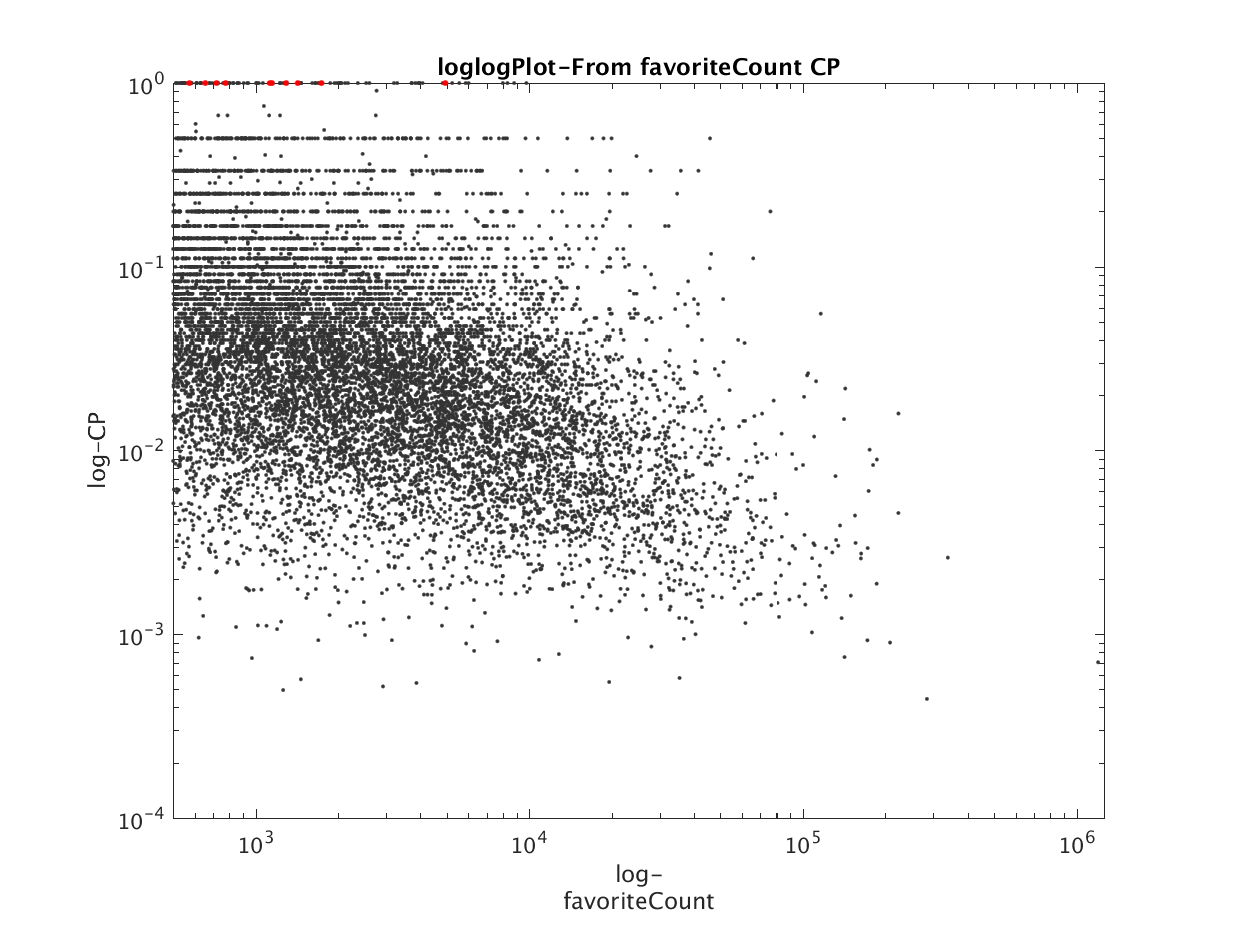
\epsfig{file=From_favoriteCount_CP_log_log_Plot.eps, height=2.5in, width=3in}
\caption{A sample scatter plot for Conditional Property of $From_user$ vs. Favorite Count (.eps format)
that has been resized with the \texttt{epsfig} command.}
\end{figure}

\subsubsection{Box Plots for Topics/Locations}
%\begin{figure}
%\centering
%\epsfig{file=fly.eps}
%\caption{A sample black and white graphic (.eps format).}
%\end{figure}

\subsubsection{Tables}

%\begin{table}
%\centering
%\caption{Frequency of Special Characters}
%\begin{tabular}{|c|c|l|} \hline
%Non-English or Math&Frequency&Comments\\ \hline
%\O & 1 in 1,000& For Swedish names\\ \hline
%$\pi$ & 1 in 5& Common in math\\ \hline
%\$ & 4 in 5 & Used in business\\ \hline
%$\Psi^2_1$ & 1 in 40,000& Unexplained usage\\
%\hline\end{tabular}
%\end{table}

%\begin{table*}
%\centering
%\caption{Some Typical Commands}
%\begin{tabular}{|c|c|l|} \hline
%Command&A Number&Comments\\ \hline
%\texttt{{\char'134}alignauthor} & 100& Author alignment\\ \hline
%\texttt{{\char'134}numberofauthors}& 200& Author enumeration\\ \hline
%\texttt{{\char'134}table}& 300 & For tables\\ \hline
%\texttt{{\char'134}table*}& 400& For wider tables\\ \hline\end{tabular}
%\end{table*}
% end the environment with {table*}, NOTE not {table}!


\section{Methodology}
\begin{itemize}
\item too hard to label tweets
\item goal is to generalize from seed set of hashtags (Snowball : LOOK AT NEWMAN)
\end{itemize}

\subsection{Learning Social Sensors}
Logistic Regression

\subsection{Baselines}
\begin{itemize}
\item random
\item top 100 tweeters of  topical tweets in train
\item top 100 mentions of topical tweets in train
\item top 100 terms of topical tweets in train
\item top 100 hashtags of topical tweets in train
\end{itemize}
Consider them as weights of 1, add up, rank the tweets

\section{Evaluation}

\subsection{Data Description}

1.4 TB of Twitter over 2 years

\subsection{Data Annotation}
\begin{itemize}
\item snowball 
\item 10 categories
\end{itemize}


\subsection*{A {\secit Caveat} for the \TeX\ Expert}
Because you have just been given permission to
use the \texttt{{\char'134}newdef} command to create a
new form, you might think you can
use \TeX's \texttt{{\char'134}def} to create a
new command: \textit{Please refrain from doing this!}
Remember that your \LaTeX\ source code is primarily intended
to create camera-ready copy, but may be converted
to other forms -- e.g. HTML. If you inadvertently omit
some or all of the \texttt{{\char'134}def}s recompilation will
be, to say the least, problematic.

\section{Related Works}
social media event can be defined as an occurrence at a certain time interval and geographical region. It can be planned or unexpected e.g, concert vs. death of a celebrity, man-made or natural e.g., parade vs. earthquake, local or global e.g., concert vs. World Peace Day. Events can further be categorized based on their target users, including individuals, government agencies concerned about natural disasters and health epidemics, marketing companies, and news websites.  Historically, event detection has been studied extensively in text mining, NLP, and IR to find events from conventional media sources such as news streams  \cite{yang}. With the growth of social media sites such as Facebook, Twitter and other microblogs, social media sites have become known as powerful communication tools for sharing and exchanging information about such events. However, event detection on social media sites is more challenging due to features such as unstructured and informal text, highly length restricted, generated by novice reporters compared to journalism-trained news editors.%, and generated in real time in many cases. 

Nevertheless, it is important to investigate event detection in social media because in comparison to traditional news blogs, social media has faster response time to events and time is money (marketing), lives (disasters), or simply relevance (new).

To see how different use cases address the aforementioned technical difficulties, we focus on the three highly studied types of event detections:
\begin{itemize}
\item \textbf{Natural Disaster Detection}

\textbf{Predictive studies on disaster} \label{FP} \cite{sandy} studied the network of users and focused on choosing the best groups of users in order to achieve lead-times i.e. faster detection of disastrous event (following the concept of "friendship paradox"\footnote{On average, most people have fewer friends than their friends have}). On the other hand, \cite{sakakiEq2} used SVM classifier for detecting earthquake and employed location estimation method such as Kalman Filtering for localizing it. \cite{sakakiEq2} extracted statistical features e.g., the number and position of words in a tweet, keyword features and word context features. These studies investigated the real-time nature of Twitter and provided promising results.
%introduced in a seminal work by \cite{feld}, showing that "your friends have more friends than you do"

\textbf{Descriptive studies on disaster} Related works discuss the behavior of Twitter users during crisis \cite{vieweg, cheong, starbird} but do not address exploiting detection of crisis events. They investigated the use of social media during crisis in order to identify information propagation properties, social behavior of users e.g. retweeting behavior, information contributing to situational awareness, and active players in communicating information. However, this behavioral information could be exploited in development of sensors.

\item \textbf{Health Epidemic Detection}

\textbf{Content-based methods} \cite{culotta} and \cite{aramaki} both tried to identify influenza-related tweets and find correlations of these tweets to CDC statistics.  Both works extracted bag-of-words as features. As for methodology, the former used single and multiple linear regression showing that multiple linear regression works better, while the latter employed SVM. Results showed high correlation of their estimation of influenza in early stages with values from U.S CDC and Japan's Infection Disease Surveillance Center.

\textbf{Structure-based method} In contrast to previous methods, \cite{garcia} focused on a structure-related technique and developed a model for contagious information diffusion in a social network. They provided a method for choosing sensor groups from friends of random sets of users to find more central individuals in order to enforce early detection.

\textbf{Hybrid method} \cite{sadilek} exploited both content and structure information. They employed a semi-supervised approach to learn a robust SVM classifier by training two classifiers on a labeled set and then applying them to non-labeled tweets . This enabled them to model the interplay of social activity, human mobility, and the spread of infectious disease in a large real-world population. Further, \cite{sadelik} identified sick individuals from the content of online communication. 
\end{itemize}
\section{Conclusions}


%ACKNOWLEDGMENTS are optional
\section{Acknowledgments}
\cite{cuiZhang}



\bibliographystyle{abbrv}
\bibliography{sigproc}  % sigproc.bib is the name of the Bibliography in this case

%\section{More Help for the Hardy}
%The acm\_proc\_article-sp document class file itself is chock-full of succinct
%and helpful comments.  If you consider yourself a moderately
%experienced to expert user of \LaTeX, you may find reading
%it useful but please remember not to change it.
\balancecolumns
% That's all folks!
\end{document}
